%-*- coding: utf-8 -*-
\documentclass{beamer}

\usepackage[frenchb]{babel}
\usepackage[T1]{fontenc}
\usepackage[utf8]{inputenc}
\graphicspath{{images/}}

\usetheme{Warsaw}

\title{Projet Vitameal}
\subtitle{Restauration en milieu hospitalier}
\author{Nicolas Symphorien, Sonia Othmani, Jean-Félix Benitez}
\institute{CNAM}
\date{12/05/2017}

\logo{
\includegraphics[height=10mm]{ipst-cnam.png}}
\setbeamertemplate{background canvas}{
\includegraphics[width=\paperwidth,height=\paperheight]{fond_200.png}} % Width pour la largeur, height pour la hauteur de l'image

\begin{document}
\begin{frame}[plain]
  \titlepage
\end{frame}

\begin{frame}
  \frametitle{Sommaire}
  \tableofcontents
\end{frame}

\section{Définition du problème}
\begin{frame}[label=definitionDuProbleme]
\frametitle{Définition du problème}
L'élaboration de menus dans un hôpital pour la restauration des patients
est une tâche complexe, et doit tenir compte des différentes pathologies
rencontrées. Faute de moyens (temps et argent) seules quelques grandes
lignes de restauration sont retenues; alors qu'idéalement, chaque
patient devrait pourvoir avoir un repas adapté à sa pathologie.
\end{frame}

\subsection{Solution envisagée}
\begin{frame}[label=solutionEnvisagée]
\frametitle{Solution envisagée}
Le projet Vitameal a pour objectif de faire correspondre au mieux la planification des régimes et des
prescriptions diététiques aux repas réellement servis au patient. Il consiste en un outil interfaçant la
gestion de production, la prise de commande et le suivi nutritionnel des repas.
\end{frame}

\subsection{Périmètre}
\begin{frame}[label=perimetre]
\frametitle{Périmètre}
C'est un diététicien qui renseigne le profil diététique des patients,
sous les directives des médecins. C'est aussi un diététicien qui élabore
les menus des patients. L'outil élaborera donc
les menus par filtrage des produits correspondants aux profils
diététiques des patients. Pour des raisons de simplifications, nous nous limiterons dans ce projet aux seuls patients adolescents et adultes, à l'exclusion des personnes agées.
\end{frame}

\section{Analyse des exigences}
\subsection{Analyse}
\begin{frame}[label=analyseDesExigences] %allowframebreaks
\frametitle{Analyse des exigences}
\begin{itemize}
  \item Partie prenantes
  \begin{itemize}
    \item Participantes~: les diététiciens, le service restauration
    \item Concernés~: les médecins, la direction (budget)
    \item Impactées~: les patients
  \end{itemize}
  \item Les besoins
  \begin{itemize}
    \item Les diététiciens renseignent les profils diététiques de chaque patient.
    \item Les diététiciens lance l'élaboration automatique des menus.
    \item Le service restauration commande les produits et ingrédients mis en œuvre dans les menus
    \item Le service restauration prépare les menus élaborés.
  \end{itemize}
  \item Les contraintes
  \begin{itemize}
    \item Les médecins doivent pouvoir vérifier / valider les profils diététiques des patients.
    \item La direction fixe un budget maximum par menu.
  \end{itemize}
\end{itemize}
\end{frame}

\subsection{Exigences}
\begin{frame}
 \frametitle{Exigences}
Chaque exigence est composée de 11 champs:
\begin{itemize}
\item \textbf{numéro:} Formé comme suit REQ\_12345
\item \textbf{Titre:} Titre ou description courte
\item \textbf{Corps:} Expression de l'exigence
\item \textbf{Type:} Utilisateur, Métier, Système, Contrainte
\item \textbf{Nature:} Fonctionnelle, Ergonomie, Robustesse, Performance, Sécurité
\item \textbf{Origine:} D'où vient une exigence ?
\item \textbf{Version:} ou niveau de maturité, Initiale, Intermédiaire, Finale
\item \textbf{Priorité:} MoSCoW, Must, Should, Could, Won't
\item \textbf{Validée:} L'exigences a-t-elle été validée ? (Oui / Non)
\item \textbf{Liens:} Liens
\item \textbf{Test:} Définition du test qui validera l'exigence.
\end{itemize}

\url{../Exigences/Exigences.html}
\end{frame}

\section{Cas d'Utilisations}
\subsection{Composer un plat}
\begin{frame}
\frametitle{Composer un plat}
\subsection{Composer les
plats}\label{diagramme-composer-les-plats}

\begin{figure}
\centering
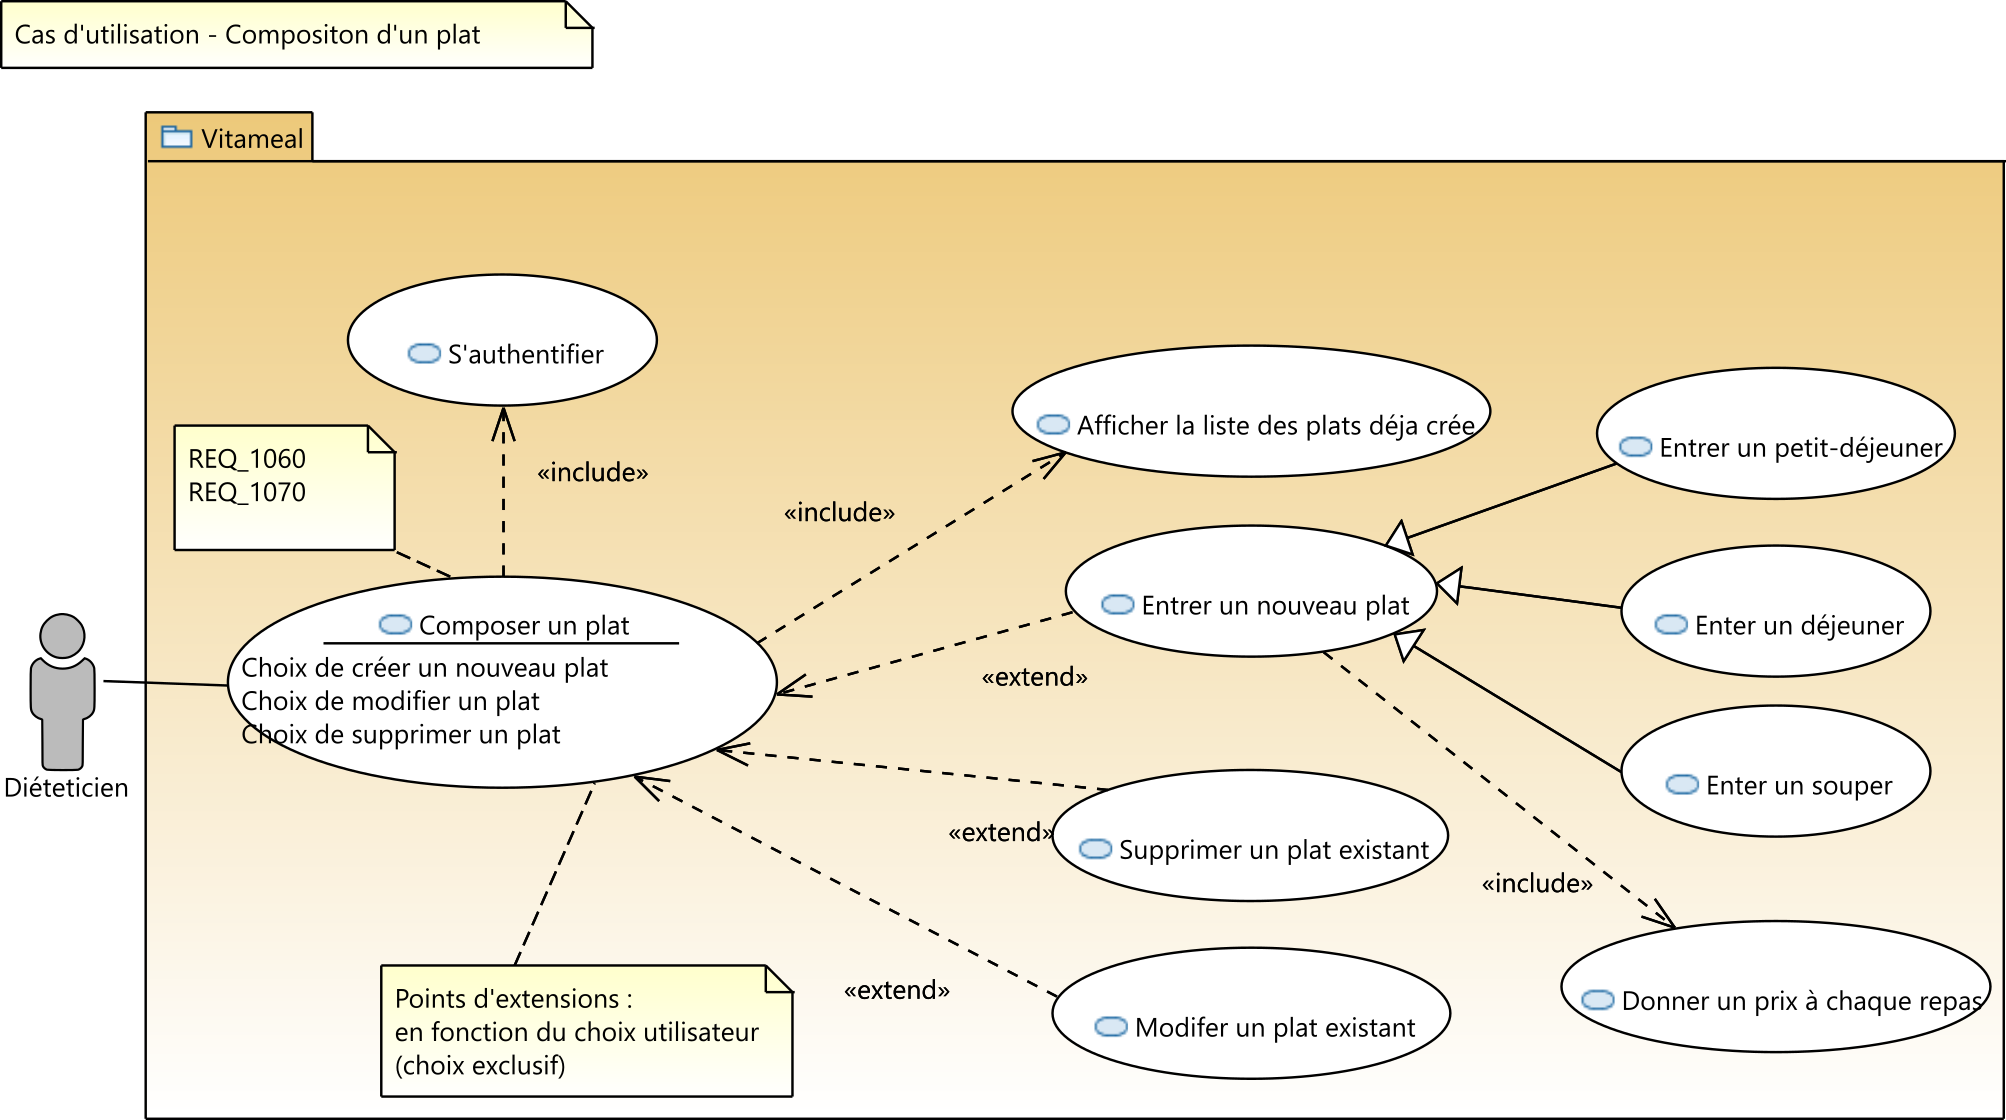
\includegraphics[width=0.9\textwidth]{../../CasDUtilisations/CompositionPlat/uc_composer_un_plat.png}
\caption{Use case composer les plats}
\end{figure}

\subsubsection{UC100 - Composer les
plats}\label{uc100---composer-les-plats}

\noindent\textbf{Nom:} Composer les plats\\
\textbf{ID:} UC100\\
\textbf{Description :} Le diététicien souhaite pouvoir élaborer les
plats composant une journée (petit-déjeuner, déjeuner, souper) en
renseignant leur compositions.\\
\textbf{Auteur :} Nicolas SYMPHORIEN\\
\textbf{Date :} 08/05/2017\\
\textbf{Acteurs :} Le diététicien\\
\textbf{Pré-condition :} L'utilisateur doit être identifié en tant que
diététicien (Voir cas d'utilisation ``S'authentifier'')

\textbf{Scénario principal:}\\
1. Le système affiche la liste des plat déjà créer 2. L'utilisateur
choisi une action :\\
a. L'utilisateur choisi de modifier un plat voir (UC101)\\
b. L'utilisateur choisi de crée un nouveau plat (UC102)\\
c. L'utilisateur choisi de supprimer un plat déjà existant (UC103) 3. Le
système renvoi vers l'écran choisi : ``Modifier un plat'', ``Créer un
plat'' ou affiche une confirmation pour la suppression d'un plat

\textbf{Scénario alternatif:}\\
1. a Le système n'obtient pas la liste des ingrédients

\textbf{Post-Conditions:} L'utilisateur est re-dirigé vers sa sélection.

\subsubsection{UC101 - Modifier un plat
existant}\label{uc101---modifier-un-plat-existant}

\noindent\textbf{Nom:} Modifier un plat existant\\
\textbf{ID:} UC101\\
\textbf{Description :} Le diététicien souhaite pouvoir modifier la
composition d'un plat.\\
\textbf{Auteur :} Nicolas SYMPHORIEN\\
\textbf{Dates :} 08/05/2017\\
\textbf{Acteurs :} Le diététicien\\
\textbf{Pré-condition :} L'utilisateur doit être identifié en tant que
diététicien (Voir cas d'utilisation ``S'authentifier'')

\textbf{Scénario principal :}\\
1. Le système restaure la composition du plat sélectionner et va à
l'étape 3 du cas d'utilisation ``Créer un nouveau plat''

\textbf{Scénario alternatif :}\\
1. a. Le système n'obtient pas la composition du plat sélectionner

\textbf{Post-Conditions:} Le plat est modifié et la modification
enregistrée

\subsubsection{UC102 - Créer un nouveau
plat}\label{uc102---cruxe9er-un-nouveau-plat}

\noindent\textbf{Nom :} Créer un nouveau plat\\
\textbf{ID :} UC102\\
\textbf{Description :} Le diététicien souhaite pouvoir créer la
composition d'un nouveau plat de type petit-déjeuner, déjeuner ou
souper.\\
\textbf{Auteur :} Nicolas SYMPHORIEN\\
\textbf{Dates :} 08/05/2017\\
\textbf{Acteurs :} Le diététicien\\
\textbf{Pré-condition :} L'utilisateur doit être identifié en tant que
diététicien (Voir cas d'utilisation ``S'authentifier'')

\textbf{Scénarios nominal :}\\
1. Le système affiche une page permettant d'entrer la composition d'un
plat 2. L'utilisateur choisi le type de plat (petit-déjeuner, déjeuner,
souper) 3. Le système propose à l'utilisateur une liste de composante à
remplir en fonction du type de plat choisie 4. L'utilisateur choisi les
ingrédients qu'il veut mettre dans chaque composantes 5. L'utilisateur
valide son choix 6. Le système enregistre le nouveau plat dans sa liste
de plats éligible a la composition des menus

\textbf{Scénarios alternatif :}

\begin{enumerate}
\def\labelenumi{\arabic{enumi}.}
\setcounter{enumi}{2}
\item
  \begin{enumerate}
  \def\labelenumii{\alph{enumii}.}
  \item
    L'utilisateur change de type de plat en cours d'élaboration\\
  \end{enumerate}
\item
  \begin{enumerate}
  \def\labelenumii{\alph{enumii}.}
  \setcounter{enumii}{1}
  \item
    Le système propose à l'utilisateur la liste de composante
    correspondante à son nouveau choix (retour etape 3.)\\
  \end{enumerate}
\item
  \begin{enumerate}
  \def\labelenumii{\alph{enumii}.}
  \setcounter{enumii}{2}
  \item
    Le système n'obtient pas la composition du liste des ingrédients\\
  \end{enumerate}
\item
  \begin{enumerate}
  \def\labelenumii{\alph{enumii}.}
  \item
    L'utilisateur annule la composition du plat
  \end{enumerate}
\end{enumerate}

\textbf{Post-Conditions:} Le plat est crée et enregistré

\subsubsection{UC103 - Supprimer un
plat}\label{uc103---supprimer-un-plat}

\noindent\textbf{Nom :} Supprimer un plat\\
\textbf{ID :} UC103\\
\textbf{Description :} Le diététicien souhaite pouvoir supprimer un
plat.\\
\textbf{Auteur :} Nicolas SYMPHORIEN\\
\textbf{Dates :} 08/05/2017\\
\textbf{Acteurs concernés :} Le diététicien\\
\textbf{Pré-condition :} L'utilisateur doit être identifié en tant que
diététicien (Voir cas d'utilisation ``S'autentifier'')

\textbf{Scénarios nominal :}

\begin{enumerate}
\def\labelenumi{\arabic{enumi}.}
\item
  Le système affiche un message d'avertissement avant la suppression
\item
  L'utilisateur confirme ou non la suppression
\item
  Le système supprime le plat de sa liste des plats
\end{enumerate}

\textbf{Scénarios alternatif :}

\begin{enumerate}
\def\labelenumi{\arabic{enumi}.}
\setcounter{enumi}{2}
\item
  \begin{enumerate}
  \def\labelenumii{\alph{enumii}.}
  \item
    Le système ne réussi pas à supprimer le plat
  \end{enumerate}
\end{enumerate}

\textbf{Post-Conditions:} Le plat est supprimé

\subsubsection{UC202 - Donner un prix à chaque
repas}\label{uc202---donner-un-prix-uxe0-chaque-repas}

\noindent\textbf{Nom :} Donner un prix à chaque repas\\
\textbf{ID :} UC202\\
\textbf{Description :} Le service restauration souhaite pouvoir donnée
le pris de chaque plat composant un menu\\
\textbf{Auteur :} Nicolas SYMPHORIEN\\
\textbf{Dates(s) :} 08/05/2017\\
\textbf{Acteurs :} Le service restauration, par héritage, le diététicien
et le médecin\\
\textbf{Pré-condition :} L'utilisateur doit être identifié

\textbf{Scénario principal :}\\
1. Le système propose de renseigner le prix du plat

\textbf{Scénario alternatif :} aucun

\textbf{Post-Conditions:} Le prix du plat est renseigné

\end{frame}

\subsection{Génération des menus}
\begin{frame}
\frametitle{Génération des menus}
%-*- coding: utf-8 -*-
\subsubsection{Élaboration des menus}
\begin{figure}
  \centering
      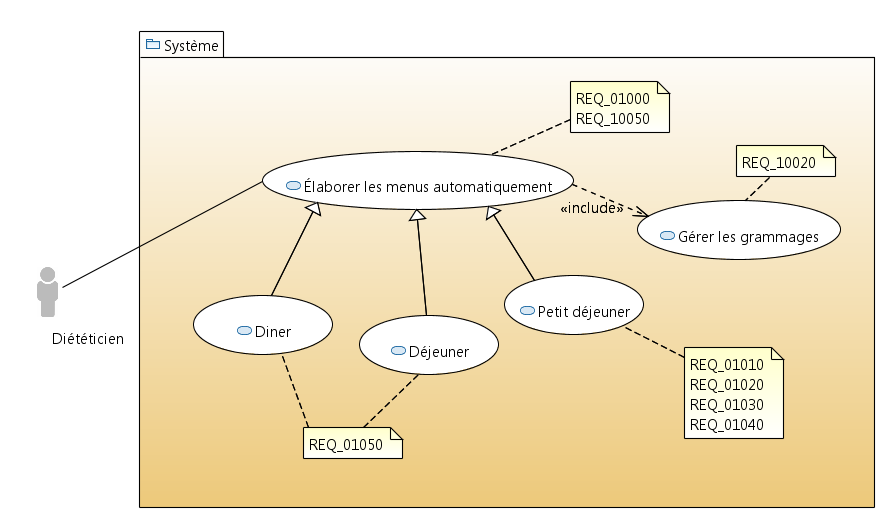
\includegraphics[width=1.00\textwidth]{../../CasDUtilisations/MenuGen/CasDUtilisation/MenuGen.png} %
\caption{Cas d'utilisation élaboration des menus}
\label{MenuGenCU}
\end{figure}

\begin{description}
\item[Nom:] Élaboration des menus (Figure \ref{MenuGenCU}).
\item[ID:] UC300
\item[Description:] Permet l'élaboration des menus.
\item[Auteur:] Jean-Félix BENITEZ.
\item[Date:] 15/06/2017
\item[Acteurs:] Diététiciens.
\item[Pré-Conditions:] Le diététicien s'est connecté au système.
\item[Scénario principal:] Figure \ref{MenuGenSeq}
  \begin{enumerate}
  \item Le diététicien sélectionne le groupe de patients pour lequel il veut générer les menus,
  \item \label{LanceElab}ensuite il lance l'élaboration des menus.
  \item L'élaboration automatique ce déroule en prenant en compte les grammages.
  \item Lorsque les menus sont élaborés, s'il estime l'élaboration correcte, il la valide.
  \item S'il estime l'élaboration incorrecte, il peut la rejeter, auquel cas il reviens à l'étape \ref{LanceElab}
  \item S'il estime l'élaboration incorrecte, il peut aussi la modifier manuellement.
  \end{enumerate}
\item[Scénario alternatif:] Aucun.
\item[Post-Conditions:] Les menus sont générés.
\end{description}

\begin{figure}
  \centering
      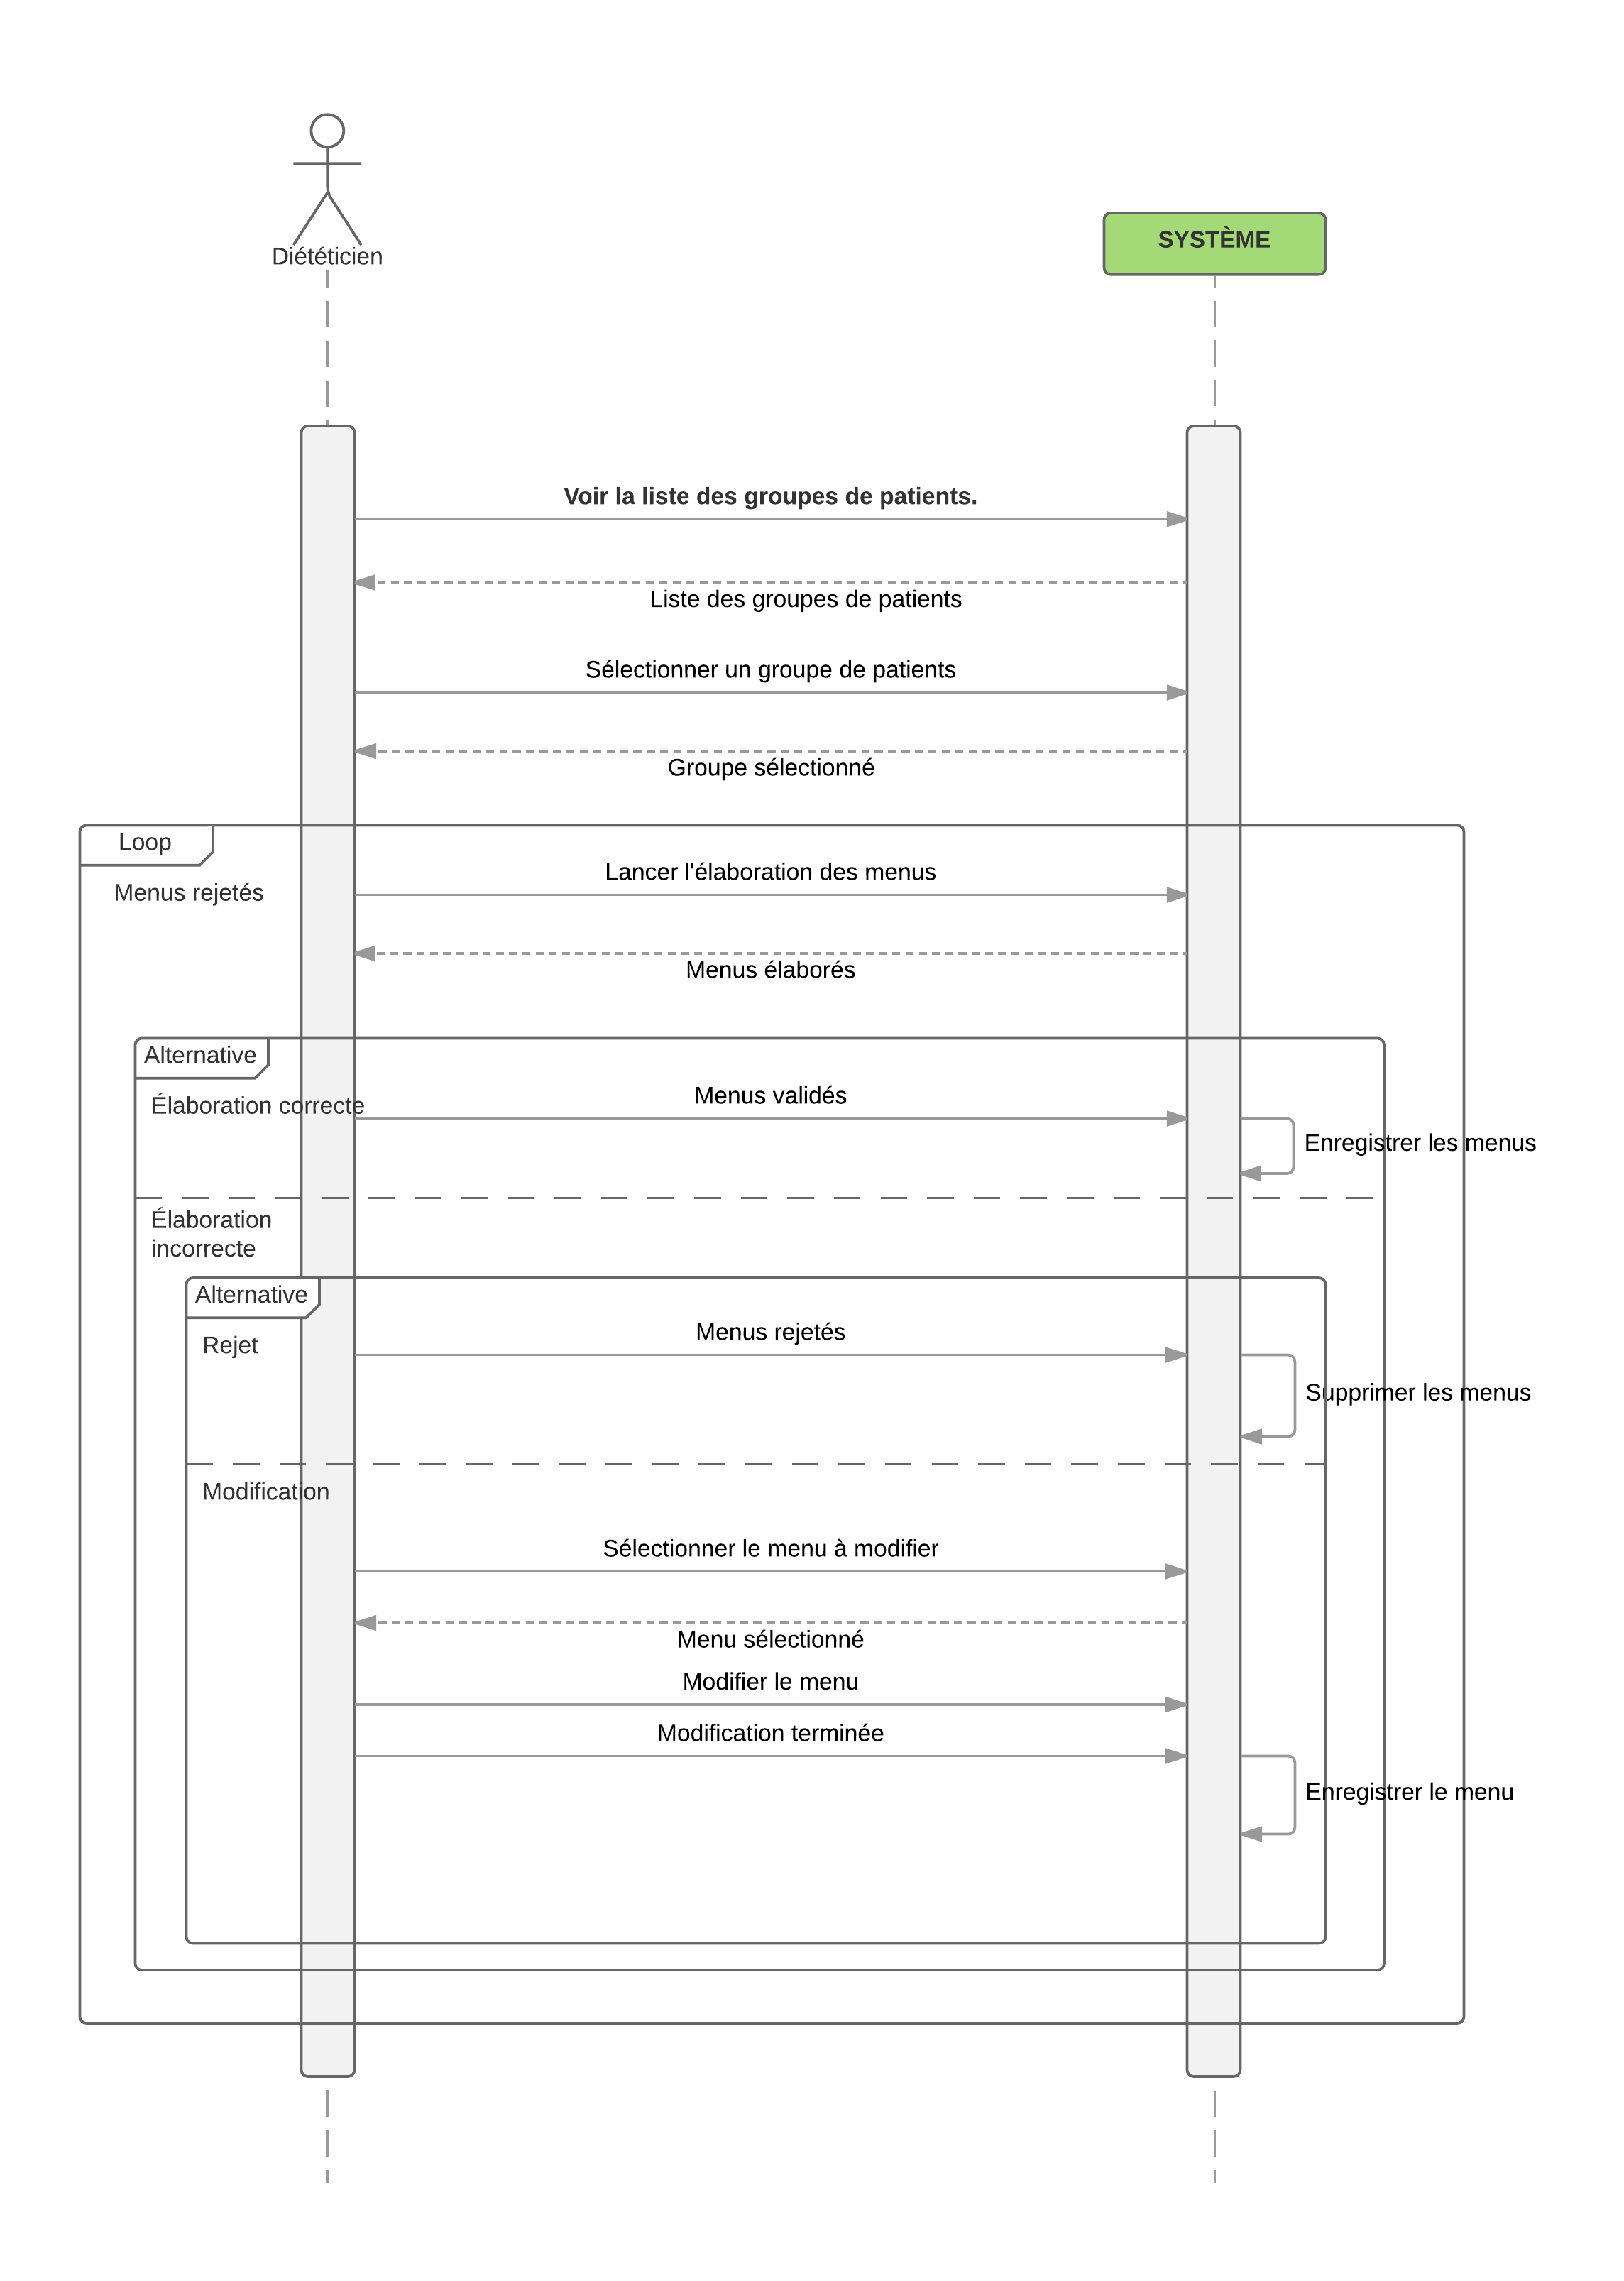
\includegraphics[width=1.00\textwidth]{../../CasDUtilisations/MenuGen/Sequence/ElaborationMenus.png} %
\caption{Séquence élaboration des menus}
\label{MenuGenSeq}
\end{figure}

\end{frame}

\subsection{Affichage des menus}
\begin{frame}
\frametitle{Affichage des menus}
\subsection{Diagramme afficher les menus
générés}\label{diagramme-afficher-les-menus-guxe9nuxe9ruxe9s}

\begin{figure}
\centering
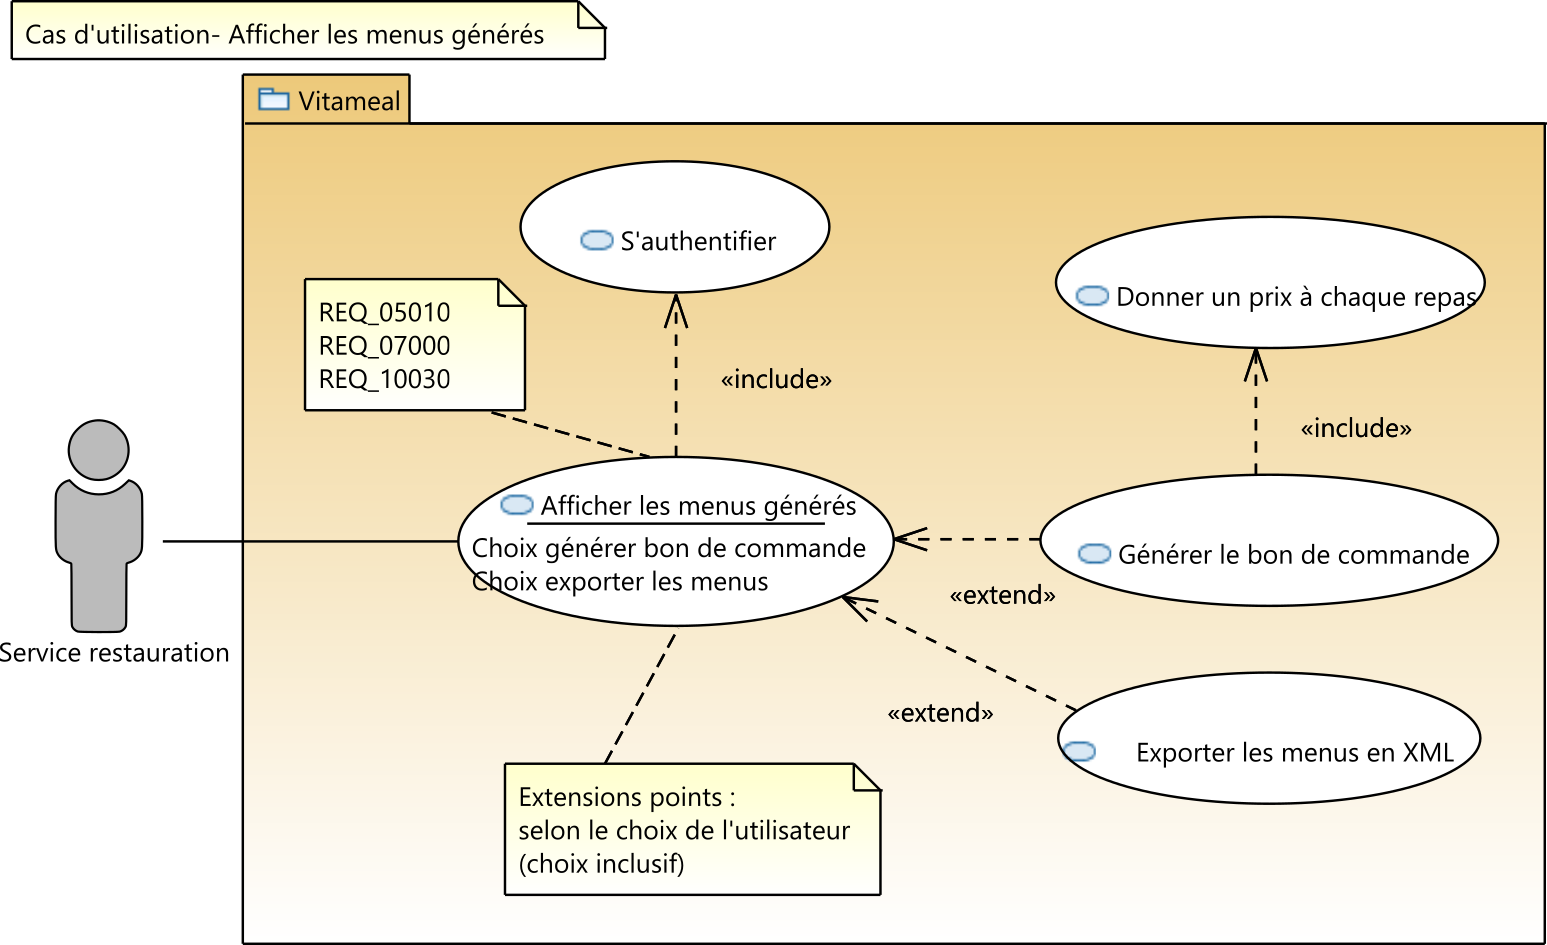
\includegraphics[width=0.85\textwidth]{../../CasDUtilisations/AfficherMenu/uc_afficher_menu.png}
\caption{Use case afficher les menus générés}
\end{figure}

\subsubsection{UC200 - Afficher les menus
générés}\label{uc200---afficher-les-menus-guxe9nuxe9ruxe9s}

\noindent\textbf{Nom :} Modifier un plat existant\\
\textbf{ID :} UC200\\
\textbf{Description :} Le service restauration souhaite pouvoir voir le
menu généré et selon son choix imprimer un bon\\
de commande et/ou exporter le menu sous un autre format.\\
\textbf{Auteur :} Nicolas SYMPHORIEN\\
\textbf{Dates(s) :} 08/05/2017\\
\textbf{Acteurs :} Le service restauration, par héritage, le diététicien
et le médecin\\
\textbf{Pré-condition :} L'utilisateur doit être identifié

\textbf{Scénario principal :}\\
1. Le système affiche un menu pour un groupe de patient donné 2.
L'utilisateur peut choisir de générer et voir le bon de commande associé
au menu affiché et l'utilisateur peut choisir de exporter le menu (pour
un usage par une tierce application)

\textbf{Scénario alternatif :}\\
1.a L'utilisateur peut changer de groupe de patient 1.b Le système
n'arrive pas à récupérer les menu générés 1.c Le système ne possède pas
de menu généré, il affiche un message d'information à l'utilisateur

\textbf{Post-Conditions:} Le menu est affiché. Un bon de commande est
produit. Un export est produit.

\subsubsection{UC201 - Générér le bon de
commande}\label{uc201---guxe9nuxe9ruxe9r-le-bon-de-commande}

\noindent\textbf{Nom :} Générer le bon de commande\\
\textbf{ID :} UC201\\
\textbf{Description :} Le service restauration souhaite pouvoir imprimer
un bon de commande du menu affiché\\
\textbf{Auteur :} Nicolas SYMPHORIEN\\
\textbf{Dates(s) :} 08/05/2017\\
\textbf{Acteurs :} Le service restauration, par héritage, le diététicien
et le médecin\\
\textbf{Pré-condition :} L'utilisateur doit être identifié

\textbf{Scénario principal :}\\
1. Le système propose la génération du menu si le prix de chaque plat a
été renseigné

\textbf{Scénario alternatif :}\\
1. a. Le prix de chaque plat n'a pas été renseigné

\textbf{Post-Conditions:} Le bon de commande et généré et affiché.

\subsubsection{UC202 - Donner un prix à chaque
repas}\label{uc202---donner-un-prix-uxe0-chaque-repas}

\noindent\textbf{Nom :} Donner un prix à chaque repas\\
\textbf{ID :} UC202\\
\textbf{Description :} Le service restauration souhaite pouvoir donnée
le pris de chaque plat composant un menu\\
\textbf{Auteur :} Nicolas SYMPHORIEN\\
\textbf{Dates(s) :} 08/05/2017\\
\textbf{Acteurs :} Le service restauration, par héritage, le diététicien
et le médecin\\
\textbf{Pré-condition :} L'utilisateur doit être identifié

\textbf{Scénario principal :}\\
1. Le système propose de renseigner le prix du plat

\textbf{Scénario alternatif :} aucun

\textbf{Post-Conditions:} Le prix du plat est renseigné

\subsubsection{UC203 - Exporter le menu affiché au format
XML}\label{uc203---exporter-le-menu-affichuxe9-au-format-xml}

\noindent\textbf{Nom :} Exporter le menu affiché au format XML\\
\textbf{ID :} UC203\\
\textbf{Description :} Le service restauration souhaite pouvoir exporté
le menu affiché pour un usage dans une tierce application (comme le site
internet de l'hopital par exemple)\\
\textbf{Auteur :} Nicolas SYMPHORIEN\\
\textbf{Dates(s) :} 08/05/2017\\
\textbf{Acteurs :} Le service restauration, par héritage, le diététicien
et le médecin\\
\textbf{Pré-condition :} L'utilisateur doit être identifié

\textbf{Scénario principal :}\\
1. Le système exporte le menu affiché en XML

\textbf{Scénario alternatif :} échec de l'export

\textbf{Post-Conditions:} Le menu est exportée au format XML

\end{frame}

\section{Planning}
\begin{frame}[label=planning]
\frametitle{Planning}
\begin{figure}[H]
\textbf{G}antt
\label{Gantt}
  \centering
      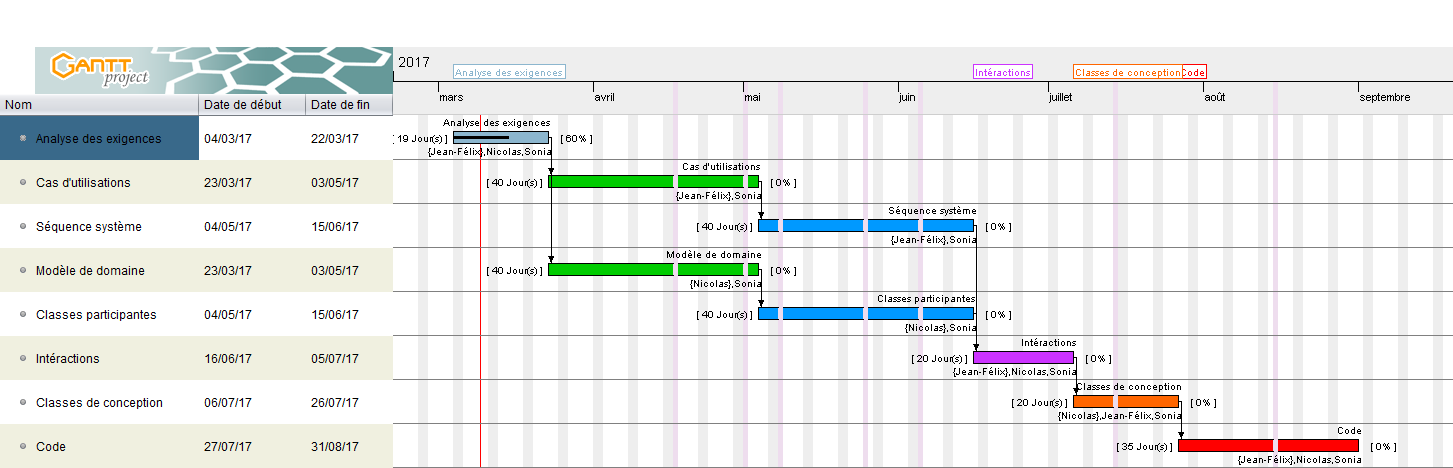
\includegraphics[width=0.95\textwidth]{Vitameal_gantt.png} %
%\caption{Gantt}
\end{figure}

\begin{figure}[H]
\textbf{P}rogram \textbf{E}valuation and \textbf{R}eview \textbf{T}echnique
\label{PERT}
  \centering
      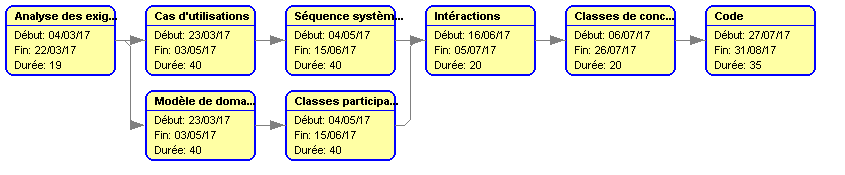
\includegraphics[width=0.95\textwidth]{Vitameal_pert.png} %
%\caption{PERT}
\end{figure}
\end{frame}

\section{Usine logicielle}
\begin{frame}[label=usineLogicielle]
\frametitle{Usine logicielle}
L'usine logicielle de Vitameal répond aux exigences suivantes :
\begin{itemize}
\item respecter les règles de qualités ;
\item avoir une documentation claire et intégrée au projet ;
\item gérer les erreurs et assurer leurs suivies ;
\item versionner le code source et la documentation ;
\item avoir un espace commun accessible à distance ;
\item gérer un espace de livraison générant des indicateurs de santé sur le projet ;
\item avoir un outil de conception UML couvrant la méthode minimal UML;
\item gérer la planification du projet.
\end{itemize}
\end{frame}

\subsection{Documentation}
\begin{frame}[label=documentation]
  \frametitle{Usine logicielle - Documentation}
  \begin{itemize}
  \item utilisation de la syntaxe \textbf{markdown};
  \item intégration à \textbf{GitHub};
  \item usage de \textbf{LaTex} pour les livrables
\end{itemize}
\end{frame}

\subsection{Poste de développement}
\begin{frame}[label=posteDeveloppement]
  \frametitle{Usine logicielle - Poste de Développement}
  \begin{itemize}
  \item \textbf{Eclipse} comme IDE pour écrire/éditer le code de l'application ;
  \item \textbf{Maven} comme constructeur du projet (gestion des dépendances, automatisation de la construction)
  \item \textbf{JUnit} pour écrire les tests unitaires de l'application et Coderturapour analyser la couverture du projet par ces tests ;
  \item \textbf{Git} pour versionnerles sources du projet ;
  \item \textbf{StarUML} pour modéliser selon le standard UML le projet ;
  \item \textbf{GanttProject} pour planifier le projet avec un diagramme de Gantt ;
  \item \textbf{TEXMaker} pour éditer les fichiers «.tex» avec un comportement proche des WYSIWYG (optionnel).
\end{itemize}  
\end{frame}

\subsection{Espace d'intégration continue}
\begin{frame}[label=integrationContinue]
  \frametitle{Usine logicielle - Espace d’intégration continue}
  \begin{itemize}
  \item \textbf{GitHub} comme gestionnaire à distance du repositorie \textbf{Git} principal, comme tracker de bug et comme affichage visuel des taches à faire ;
  \item \textbf{Jenkins} comme serveur d'intégration continue ;
  \item \textbf{SonarQube} comme analyseur de qualité du code.
  \end{itemize}
\end{frame}

\subsection{Schéma de fonctionnement}
\begin{frame}[label=schemaFonctionnement]
  \frametitle{Usine logicielle - Schéma de fonctionnement}
\begin{figure}[H]
\label{schema}
  \centering
      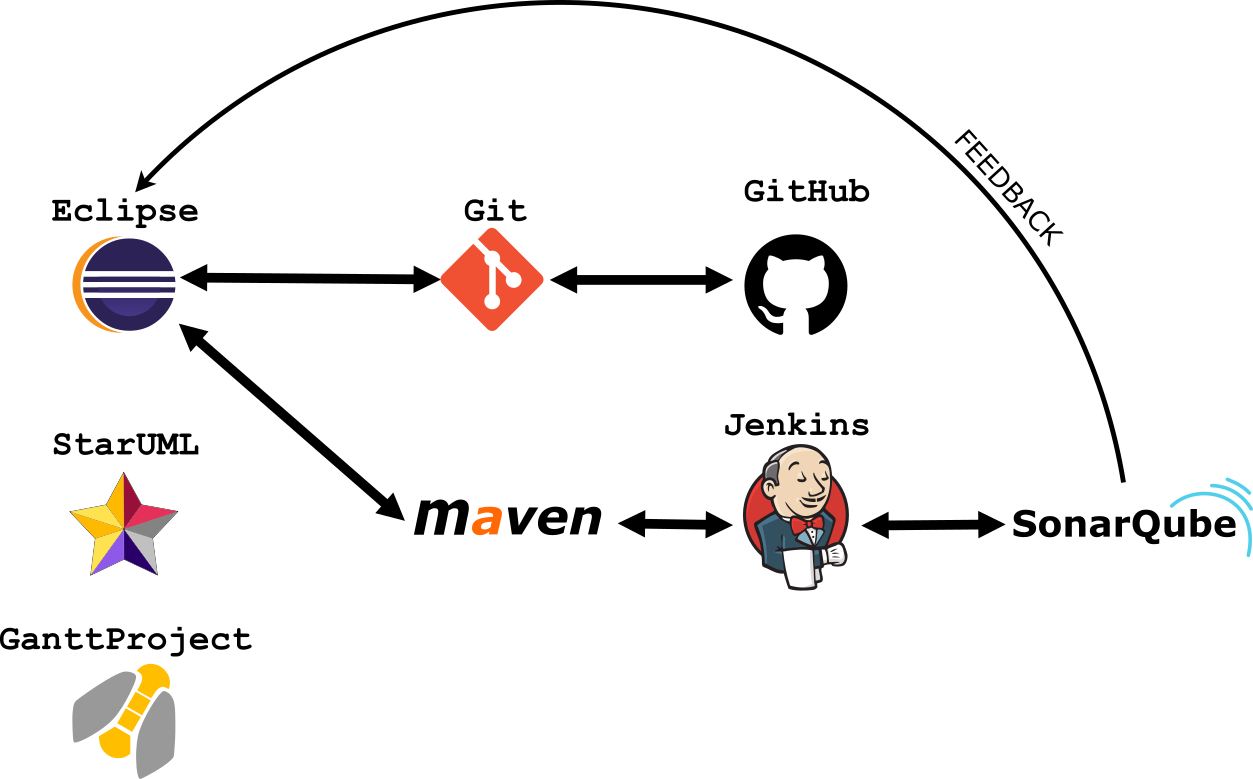
\includegraphics[width=1.0\textwidth]{usine_vitameal.png} %
%\caption{Schéma}
\end{figure}
\end{frame}

\end{document}
